%  LaTeX support: latex@mdpi.com 
%  For support, please attach all files needed for compiling as well as the log file, and specify your operating system, LaTeX version, and LaTeX editor.

\newcommand{\qsdpapertitle}{Causal Motion Under Planck-Paced Reconfiguration: Inertial Emergence in General Substrate Theory}
\newcommand{\qsdauthorname}{Michael Bush}
\newcommand{\qsdauthorinitials}{M.B.}
\newcommand{\qsdauthoremail}{mbush@haddentechnologies.com}
\newcommand{\qsdorcid}{0009-0003-9747-9109}
\newcommand{\qsdcorp}{Hadden Technologies Corporation}
\newcommand{\qsdgptname}{ChatGPT}
\newcommand{\qsdgptver}{GPT-4o}
\newcommand{\qsdgptyear}{2025}
\newcommand{\qsdkeywords}{General Substrate Theroy,GST,Quantum Substrate Dynamics,QSD,Inertia,Scalar coherence,Substrate dynamics,planck energy,
Phase re-locking,Momentum,Rotational loss,Scalar recovery,Mass-phase,Conserved substrate}
\newcommand{\qsdmethodstatement}
{This work was developed through first-principles modeling using a conserved coherence substrate framework. All derivations were performed structurally, with motion, inertia, and rotational behavior treated as manifestations of scalar phase reconfiguration. Mathematical relationships were constructed to maintain causal consistency and empirical compatibility, while avoiding reliance on classical axioms such as intrinsic mass or force. The method emphasizes substrate conservation, phase continuity, and Lorentz-invariant scalar timing to reveal the structural origins of inertial and dynamic behavior.}
\newcommand{\qsdabstract}
{This paper presents a structural reinterpretation of motion, inertia, and momentum under the General Substrate Theory (GST), in which all physical evolution is governed by the Substrate Response Law (SRL). Within this framework, Quantum Substrate Dynamics (QSD) models motion not as spatial traversal, but as scalar-paced reconfiguration of coherence structures embedded in a conserved substrate. Coherence transport is constrained by a minimum causal interval—the Planck-scale tick—defining the maximum rate at which coherence structures can re-lock across the substrate.  
\\
In this view, velocity does not alter the size of the coherence envelope ($L_{\text{coh}}$); instead, it compresses coherence content (increases scalar coherence density) within the fixed spatial envelope. This coherence-density compression sets a fundamental mass–velocity limit: even in uniform motion, a maximum scalar coherence density is reached before the scalar recovery speed ($c_s$), causing collapse or scalar offload. Inertia thus emerges naturally from delayed scalar re-locking under coherence deformation, and momentum reflects the substrate’s structural commitment to maintaining a phase-preserving trajectory across sequential causal intervals. Uniform motion corresponds to tension-neutral phase continuity, while acceleration, deceleration, and rotation invoke scalar recovery work—producing observable thermal and kinetic signatures. Rotational motion is inherently lossy due to persistent phase curvature, and gyroscopic resistance is derived from the substrate’s conservation of angular coherence memory. Weight is reframed as scalar pushback arising from denied re-locking into a gravitational tension gradient.
\\
No classical law is violated; each is reinterpreted as a regime-specific expression of structural tension and coherence compression under causal pacing. In this model, motion, inertia, and momentum emerge not from force or intrinsic mass, but from substrate geometry, scalar reconfiguration timing, and structural conservation. The result is a physically grounded, falsifiable alternative to classical mechanics—one that enables new approaches to transport, thermal asymmetry, and inertial design within a causally constrained coherence substrate.}

%=================================================================
\documentclass[preprints,article,submit,pdftex,moreauthors]{Definitions/mdpi} 
%\documentclass[preprints,article,submit,pdftex,moreauthors]{Definitions/mdpi} 
% For posting an early version of this manuscript as a preprint, you may use "preprints" as the journal. Changing "submit" to "accept" before posting will remove line numbers.

% Below journals will use APA reference format:
% admsci, aieduc, behavsci, businesses, econometrics, economies, education, ejihpe, famsci, games, humans, ijcs, ijfs, journalmedia, jrfm, languages, psycholint, publications, tourismhosp, youth

% Below journals will use Chicago reference format:
% arts, genealogy, histories, humanities, jintelligence, laws, literature, religions, risks, socsci

%--------------------
% Class Options:
%--------------------
%----------
% journal
%----------
% Choose between the following MDPI journals:
% accountaudit, acoustics, actuators, addictions, adhesives, admsci, adolescents, aerobiology, aerospace, agriculture, agriengineering, agrochemicals, agronomy, ai, air, algorithms, allergies, alloys, amh, analytica, analytics, anatomia, anesthres, animals, antibiotics, antibodies, antioxidants, applbiosci, appliedchem, appliedmath, appliedphys, applmech, applmicrobiol, applnano, applsci, aquacj, architecture, arm, arthropoda, arts, asc, asi, astronomy, atmosphere, atoms, audiolres, automation, axioms, bacteria, batteries, bdcc, behavsci, beverages, biochem, bioengineering, biologics, biology, biomass, biomechanics, biomed, biomedicines, biomedinformatics, biomimetics, biomolecules, biophysica, biosensors, biosphere, biotech, birds, blockchains, bloods, blsf, brainsci, breath, buildings, businesses, cancers, carbon, cardiogenetics, catalysts, cells, ceramics, challenges, chemengineering, chemistry, chemosensors, chemproc, children, chips, cimb, civileng, cleantechnol, climate, clinbioenerg, clinpract, clockssleep, cmd, cmtr, coasts, coatings, colloids, colorants, commodities, complications, compounds, computation, computers, condensedmatter, conservation, constrmater, cosmetics, covid, crops, cryo, cryptography, crystals, csmf, ctn, curroncol, cyber, dairy, data, ddc, dentistry, dermato, dermatopathology, designs, devices, diabetology, diagnostics, dietetics, digital, disabilities, diseases, diversity, dna, drones, dynamics, earth, ebj, ecm, ecologies, econometrics, economies, education, eesp, ejihpe, electricity, electrochem, electronicmat, electronics, encyclopedia, endocrines, energies, eng, engproc, ent, entomology, entropy, environments, epidemiologia, epigenomes, esa, est, famsci, fermentation, fibers, fintech, fire, fishes, fluids, foods, forecasting, forensicsci, forests, fossstud, foundations, fractalfract, fuels, future, futureinternet, futureparasites, futurepharmacol, futurephys, futuretransp, galaxies, games, gases, gastroent, gastrointestdisord, gastronomy, gels, genealogy, genes, geographies, geohazards, geomatics, geometry, geosciences, geotechnics, geriatrics, glacies, grasses, greenhealth, gucdd, hardware, hazardousmatters, healthcare, hearts, hemato, hematolrep, heritage, higheredu, highthroughput, histories, horticulturae, hospitals, humanities, humans, hydrobiology, hydrogen, hydrology, hygiene, idr, iic, ijerph, ijfs, ijgi, ijmd, ijms, ijns, ijpb, ijt, ijtm, ijtpp, ime, immuno, informatics, information, infrastructures, inorganics, insects, instruments, inventions, iot, j, jal, jcdd, jcm, jcp, jcs, jcto, jdad, jdb, jeta, jfb, jfmk, jimaging, jintelligence, jlpea, jmahp, jmmp, jmms, jmp, jmse, jne, jnt, jof, joitmc, joma, jop, jor, journalmedia, jox, jpbi, jpm, jrfm, jsan, jtaer, jvd, jzbg, kidney, kidneydial, kinasesphosphatases, knowledge, labmed, laboratories, land, languages, laws, life, lights, limnolrev, lipidology, liquids, literature, livers, logics, logistics, lubricants, lymphatics, machines, macromol, magnetism, magnetochemistry, make, marinedrugs, materials, materproc, mathematics, mca, measurements, medicina, medicines, medsci, membranes, merits, metabolites, metals, meteorology, methane, metrics, metrology, micro, microarrays, microbiolres, microelectronics, micromachines, microorganisms, microplastics, microwave, minerals, mining, mmphys, modelling, molbank, molecules, mps, msf, mti, multimedia, muscles, nanoenergyadv, nanomanufacturing, nanomaterials, ncrna, ndt, network, neuroglia, neurolint, neurosci, nitrogen, notspecified, nursrep, nutraceuticals, nutrients, obesities, oceans, ohbm, onco, oncopathology, optics, oral, organics, organoids, osteology, oxygen, parasites, parasitologia, particles, pathogens, pathophysiology, pediatrrep, pets, pharmaceuticals, pharmaceutics, pharmacoepidemiology, pharmacy, philosophies, photochem, photonics, phycology, physchem, physics, physiologia, plants, plasma, platforms, pollutants, polymers, polysaccharides, populations, poultry, powders, preprints, proceedings, processes, prosthesis, proteomes, psf, psych, psychiatryint, psychoactives, psycholint, publications, purification, quantumrep, quaternary, qubs, radiation, reactions, realestate, receptors, recycling, regeneration, religions, remotesensing, reports, reprodmed, resources, rheumato, risks, robotics, rsee, ruminants, safety, sci, scipharm, sclerosis, seeds, sensors, separations, sexes, signals, sinusitis, siuj, skins, smartcities, sna, societies, socsci, software, soilsystems, solar, solids, spectroscj, sports, standards, stats, std, stresses, surfaces, surgeries, suschem, sustainability, symmetry, synbio, systems, tae, targets, taxonomy, technologies, telecom, test, textiles, thalassrep, therapeutics, thermo, timespace, tomography, tourismhosp, toxics, toxins, transplantology, transportation, traumacare, traumas, tropicalmed, universe, urbansci, uro, vaccines, vehicles, venereology, vetsci, vibration, virtualworlds, viruses, vision, waste, water, wem, wevj, wild, wind, women, world, youth, zoonoticdis

%---------
% article
%---------
% The default type of manuscript is "article", but can be replaced by: 
% abstract, addendum, article, benchmark, book, bookreview, briefcommunication, briefreport, casereport, changes, clinicopathologicalchallenge, comment, commentary, communication, conceptpaper, conferenceproceedings, correction, conferencereport, creative, datadescriptor, discussion, entry, expressionofconcern, extendedabstract, editorial, essay, erratum, fieldguide, hypothesis, interestingimages, letter, meetingreport, monograph, newbookreceived, obituary, opinion, proceedingpaper, projectreport, reply, retraction, review, perspective, protocol, shortnote, studyprotocol, supfile, systematicreview, technicalnote, viewpoint, guidelines, registeredreport, tutorial,  giantsinurology, urologyaroundtheworld
% supfile = supplementary materials

%----------
% submit
%----------
% The class option "submit" will be changed to "accept" by the Editorial Office when the paper is accepted. This will only make changes to the frontpage (e.g., the logo of the journal will get visible), the headings, and the copyright information. Also, line numbering will be removed. Journal info and pagination for accepted papers will also be assigned by the Editorial Office.

%------------------
% moreauthors
%------------------
% If there is only one author the class option oneauthor should be used. Otherwise use the class option moreauthors.

%---------
% pdftex
%---------
% The option pdftex is for use with pdfLaTeX. Remove "pdftex" for (1) compiling with LaTeX & dvi2pdf (if eps figures are used) or for (2) compiling with XeLaTeX.

%=================================================================
% MDPI internal commands - do not modify
\firstpage{1} 
\makeatletter 
\setcounter{page}{\@firstpage} 
\makeatother
\pubvolume{1}
\issuenum{1}
\articlenumber{0}
\pubyear{2025}
\copyrightyear{2025}
%\externaleditor{Firstname Lastname} % More than 1 editor, please add `` and '' before the last editor name
\datereceived{ } 
\daterevised{ } % Comment out if no revised date
\dateaccepted{ } 
\datepublished{ } 
%\datecorrected{} % For corrected papers: "Corrected: XXX" date in the original paper.
%\dateretracted{} % For retracted papers: "Retracted: XXX" date in the original paper.
\hreflink{https://doi.org/} % If needed use \linebreak
%\doinum{}
%\pdfoutput=1 % Uncommented for upload to arXiv.org
%\CorrStatement{yes}  % For updates
%\longauthorlist{yes} % For many authors that exceed the left citation part

%=================================================================
% Add packages and commands here. The following packages are loaded in our class file: fontenc, inputenc, calc, indentfirst, fancyhdr, graphicx, epstopdf, lastpage, ifthen, float, amsmath, amssymb, lineno, setspace, enumitem, mathpazo, booktabs, titlesec, etoolbox, tabto, xcolor, colortbl, soul, multirow, microtype, tikz, totcount, changepage, attrib, upgreek, array, tabularx, pbox, ragged2e, tocloft, marginnote, marginfix, enotez, amsthm, natbib, hyperref, cleveref, scrextend, url, geometry, newfloat, caption, draftwatermark, seqsplit
% cleveref: load \crefname definitions after \begin{document}

\usepackage{tikz}
\usetikzlibrary{angles, quotes}
\usepackage{pgfplots}
\pgfplotsset{compat=1.17}

%=================================================================
% Please use the following mathematics environments: Theorem, Lemma, Corollary, Proposition, Characterization, Property, Problem, Example, ExamplesandDefinitions, Hypothesis, Remark, Definition, Notation, Assumption
%% For proofs, please use the proof environment (the amsthm package is loaded by the MDPI class).

%=================================================================
% Full title of the paper (Capitalized)
\Title{\qsdpapertitle}


% MDPI internal command: Title for citation in the left column
\TitleCitation{Title}

% Author Orchid ID: enter ID or remove command
\newcommand{\orcidauthorA}{\qsdorcid} % Add \orcidA{} behind the author's name
%\newcommand{\orcidauthorB}{0000-0000-0000-000X} % Add \orcidB{} behind the author's name

% Authors, for the paper (add full first names)
\Author{\qsdauthorname $^{1}$\orcidA{}}

%\longauthorlist{yes}

% MDPI internal command: Authors, for metadata in PDF
\AuthorNames{\qsdauthorname}

% MDPI internal command: Authors, for citation in the left column, only choose below one of them according to the journal style
% If this is a Chicago style journal 
% (arts, genealogy, histories, humanities, jintelligence, laws, literature, religions, risks, socsci): 
% Lastname, Firstname, Firstname Lastname, and Firstname Lastname.

% If this is a APA style journal 
% (admsci, behavsci, businesses, econometrics, economies, education, ejihpe, games, humans, ijfs, journalmedia, jrfm, languages, psycholint, publications, tourismhosp, youth): 
% Lastname, F., Lastname, F., \& Lastname, F.

% If this is a ACS style journal (Except for the above Chicago and APA journals, all others are in the ACS format): 
% Lastname, F.; Lastname, F.; Lastname, F.
\isAPAStyle{%
       \AuthorCitation{Lastname, F., Lastname, F., \& Lastname, F.}
         }{%
        \isChicagoStyle{%
        \AuthorCitation{Lastname, Firstname, Firstname Lastname, and Firstname Lastname.}
        }{
        \AuthorCitation{Lastname, F.; Lastname, F.; Lastname, F.}
        }
}

% Affiliations / Addresses (Add [1] after \address if there is only one affiliation.)
\address{%
$^{1}$ \quad \qsdcorp; \qsdauthoremail\\
%$^{2}$ \quad Affiliation 2; e-mail@e-mail.com
}

% Contact information of the corresponding author
\corres{Correspondence: \qsdauthoremail (\qsdauthorinitials)}

% Current address and/or shared authorship
%\firstnote{Shiloh, IL: Independent Researcher.}  % Current address should not be the same as any items in the Affiliation section.
%\secondnote{These authors contributed equally to this work.}
% The commands \thirdnote{} till \eighthnote{} are available for further notes

%\simplesumm{} % Simple summary

%\conference{} % An extended version of a conference paper


% Abstract (Do not insert blank lines, i.e. \\) 
\abstract{\qsdabstract}

% Keywords
\keyword{\qsdkeywords} 

% The fields PACS, MSC, and JEL may be left empty or commented out if not applicable
%\PACS{J0101}
%\MSC{}
%\JEL{}

%%%%%%%%%%%%%%%%%%%%%%%%%%%%%%%%%%%%%%%%%%
% Only for the journal Diversity
%\LSID{\url{http://}}

%%%%%%%%%%%%%%%%%%%%%%%%%%%%%%%%%%%%%%%%%%
% Only for the journal Applied Sciences
%\featuredapplication{Authors are encouraged to provide a concise description of the specific application or a potential application of the work. This section is not mandatory.}
%%%%%%%%%%%%%%%%%%%%%%%%%%%%%%%%%%%%%%%%%%

%%%%%%%%%%%%%%%%%%%%%%%%%%%%%%%%%%%%%%%%%%
% Only for the journal Data
%\dataset{DOI number or link to the deposited data set if the data set is published separately. If the data set shall be published as a supplement to this paper, this field will be filled by the journal editors. In this case, please submit the data set as a supplement.}
%\datasetlicense{License under which the data set is made available (CC0, CC-BY, CC-BY-SA, CC-BY-NC, etc.)}

%%%%%%%%%%%%%%%%%%%%%%%%%%%%%%%%%%%%%%%%%%
% Only for the journal BioTech, Fishes, Neuroimaging and Toxins
%\keycontribution{The breakthroughs or highlights of the manuscript. Authors can write one or two sentences to describe the most important part of the paper.}

%%%%%%%%%%%%%%%%%%%%%%%%%%%%%%%%%%%%%%%%%%
% Only for the journal Encyclopedia
%\encyclopediadef{For entry manuscripts only: please provide a brief overview of the entry title instead of an abstract.}

%%%%%%%%%%%%%%%%%%%%%%%%%%%%%%%%%%%%%%%%%%
% Only for the journal Advances in Respiratory Medicine, Future, Sensors and Smart Cities
%\addhighlights{yes}
%\renewcommand{\addhighlights}{%
%
%\noindent This is an obligatory section in ``Advances in Respiratory Medicine'', ``Future'', ``Sensors'' and ``Smart Cities”, whose goal is to increase the discoverability and readability of the article via search engines and other scholars. Highlights should not be a copy of the abstract, but a simple text allowing the reader to quickly and simplified find out what the article is about and what can be cited from it. Each of these parts should be devoted up to 2~bullet points.\vspace{3pt}\\
%\textbf{What are the main findings?}
% \begin{itemize}[labelsep=2.5mm,topsep=-3pt]
% \item First bullet.
% \item Second bullet.
% \end{itemize}\vspace{3pt}
%\textbf{What is the implication of the main finding?}
% \begin{itemize}[labelsep=2.5mm,topsep=-3pt]
% \item First bullet.
% \item Second bullet.
% \end{itemize}
%}

%%%%%%%%%%%%%%%%%%%%%%%%%%%%%%%%%%%%%%%%%%
\begin{document}
%%%%%%%%%%%%%%%%%%%%%%%%%%%%%%%%%%%%%%%%%%
% The order of the section titles is different for some journals. Please refer to the "Instructions for Authors” on the journal homepage.

%%%%%%%%%%%%%%%%%%%%%%%%%%%%%%%%%%%%%%%%%%
\section{Introduction}
Motion is one of the most foundational concepts in physics, yet its physical origin remains unexplained. We describe velocity, acceleration, and momentum with confidence, but typically treat motion as spatial traversal, inertia as intrinsic resistance, and momentum as a quantity carried by mass. These assumptions are useful—and in practice, highly predictive—but they are not explanatory. We accept that mass resists acceleration, that moving bodies remain in motion, and that rotating systems resist tilt, without identifying what physically enforces these behaviors.

Einstein recognized this hidden substrate in his own way. The indistinguishability of rest and uniform motion, and the universality of inertial resistance, were elevated to foundational principles—but never mechanistically derived. Even today, inertia remains unexplained: not in the mathematical sense, but in the physical. What resists acceleration? Where is that resistance stored? Why is motion preserved effortlessly—until it changes?

This paper proposes that answers to these questions lie not in discarding physics, but in descending beneath it. Using the framework of General Substrate Theory (GST) and its dynamic model, Quantum Substrate Dynamics (QSD)~\cite{bush2025,bush-planck-2025,bush-coherence,bush-planck-ep}, we reinterpret motion not as geometric translation, but as scalar-paced reconfiguration of coherent structure within a conserved substrate. In this model, mass is not substance, but a phase-stable coherence knot embedded in the substrate. Motion becomes the process of continuously re-locking this coherence structure across adjacent substrate regions, constrained by a minimum causal interval—the Planck-scale tick. Crucially, velocity does not alter the spatial size of the coherence envelope ($L_{\text{coh}}$). Instead, velocity increases scalar coherence density—compressing the internal coherence content within the fixed and invariant $L_{\text{coh}}$. As a result, even uniform motion imposes a fundamental mass–velocity threshold at which coherence density reaches a maximum permissible limit, defined by the scalar recovery speed ($c_s$), beyond which structural collapse or scalar offload inevitably occurs. 

Inertia, within this framework, emerges naturally from delayed scalar re-locking under coherence deformation, while momentum represents the substrate’s structural commitment to a specific coherence-maintaining path across sequential causal intervals. Uniform motion corresponds directly to tension-neutral scalar continuity, while acceleration, deceleration, and rotation require additional scalar recovery effort—manifesting physically as observable thermal and kinetic signatures. Rotational motion, in particular, is inherently lossy due to persistent phase curvature, and gyroscopic resistance emerges structurally from the substrate’s conservation of angular coherence memory. Weight is similarly reframed as scalar pushback arising from structurally denied re-locking into a gravitational tension gradient.

Throughout this paper, we develop a first-principles derivation of motion, inertia, and momentum based solely upon structural conservation, causal pacing, and coherence continuity. No classical laws are violated; rather, each is reinterpreted as a regime-specific summary of structural tension under substrate-defined causal constraints. Newton’s equations, Einstein’s relativistic invariants, and standard field-theoretic behaviors all emerge naturally as effective expressions of this deeper substrate logic. The result is a physically grounded, falsifiable alternative to classical mechanics—one that enables novel approaches to transport, thermal asymmetry, and inertial design within a causally constrained coherence substrate.

While the framework developed here is grounded in substrate-level modeling, it resonates strongly with observed phenomena. Inertial frame equivalence and gravitational time dilation—such as those directly observed in the Global Positioning System (GPS)~\cite{ashby-gps}—naturally emerge as scalar pacing and coherence-alignment effects. Rotational decay and frame-dragging in gyroscopic systems~\cite{gp-b} strongly suggest angular coherence tension within the substrate. Even measurable thermal dissipation in rotating systems~\cite{rotational-heating} can be structurally attributed to scalar offload mechanisms predicted explicitly by this model. These empirical connections, while illustrative, underscore the compatibility of QSD with observations across both classical and relativistic domains.






%%%%%%%%%%%%%%%%%%%%%%%%%%%%%%%%%%%%%%%%%%
\section{Materials and Methods}
%%%%%%%%%%%%%%%%%%%%%%%%%%%%%%%%%%%%%%%%%%
\qsdmethodstatement
In support of the editorial process, generative AI tools—specifically OpenAI's \qsdgptname (version \qsdgptver, \qsdgptyear)—were used to assist in:
\begin{itemize}
    \item Generating illustrative figures based on the author’s conceptual framework, with iterative refinement to ensure fidelity to the substrate-based dynamics of the model,
    \item Researching, validating, and cross-referencing related scientific concepts to improve accuracy, contextual alignment, and clarity,
    \item Summarizing and formatting externally sourced material already selected by the author.
\end{itemize}

No original theoretical contributions were generated by the AI system; all scientific claims, hypotheses, derivations, and interpretations were authored and reviewed by the human researcher. The use of AI is disclosed in alignment with journal policy for transparency in the writing process.

%%%%%%%%%%%%%%%%%%%%%%%%%%%%%%%%%%%%%%%%%%
%\section{Results}

%%%%%%%%%%%%%%%%%%%%%%%%%%%%%%%%%%%%%%%%%%
\section{Discussion}
%%%%%%%%%%%%%%%%%%%%%%%%%%%%%%%%%%%%%%%%%%
\subsection{Substrate Ontology of Motion}

Under the framework of General Substrate Theory (GST), all physical evolution is governed by the Substrate Response Law (SRL): structure may only evolve as fast as the substrate can coherently re-lock it. Quantum Substrate Dynamics (QSD) interprets motion not as traversal through geometric space, but as a scalar-paced sequence of coherent structural re-locking events within a conserved substrate. Coherence transport is thus governed by a fundamental causal interval---the Planck-scale tick---which sets the pacing limit at which coherence can re-lock into adjacent substrate regions.

In this formulation, velocity does not alter the spatial extent of the coherence envelope ($L_{\text{coh}}$). Instead, velocity compresses the scalar coherence content, increasing the coherence density within the fixed envelope size. Therefore, even uniform motion places a constraint on the maximum allowed mass--velocity combination: at sufficiently high velocities, coherence density compression will eventually reach a critical scalar pacing limit, defined by the substrate's scalar recovery speed ($c_s$), causing structural collapse or scalar offload. The spatial extent of the coherence envelope $L_{\text{coh}}$ itself is influenced not by velocity but by local substrate conditions—particularly scalar tension gradients, substrate curvature, and coherence stress distributions.

In this view, velocity emerges structurally as a scalar pacing relationship between coherence envelope size and the scalar recovery interval. A structure at rest is one whose coherence boundary remains phase-stable and stationary; a structure in uniform motion re-locks coherently at a constant scalar pacing rate along a tension-neutral substrate gradient. Acceleration and deceleration, by contrast, require changes in coherence configuration and scalar pacing demands, resulting in boundary deformation, scalar recovery lag, and measurable thermal and kinetic signatures.

Space and time, therefore, are no longer fundamental coordinates but emergent substrate-level phenomena arising from scalar pacing constraints and coherence continuity. Spatial displacement corresponds directly to the successful scalar-paced re-locking of coherent structures into sequential adjacent substrate regions; temporal progression emerges inherently from the scalar recovery intervals that separate permissible re-lock events. Thus, time is structurally directional and discrete, governed explicitly by scalar pacing constraints rather than continuous geometric parameters.

The substrate itself does not flow or move; it provides a stationary, causally governed scaffold that only deforms under scalar coherence strain. Motion thus arises explicitly as a scalar-mediated reconfiguration of coherence structure, rather than passive traversal through geometric space. Classical concepts—velocity, momentum, and acceleration—are reframed as emergent summaries of this deeper scalar-guided structural realignment.

This structural ontology naturally leads to the definition of a \emph{coherence transport velocity}, representing the maximum permissible rate at which a phase-locked structure can coherently re-lock into adjacent substrate regions:

\begin{equation}
    v_{\text{coh}} = \frac{L_{\text{coh}}}{t_{\text{tick}}},
\end{equation}

where \( L_{\text{coh}} \) is the substrate-defined coherence envelope size, and \( t_{\text{tick}} = L_{\text{coh}}/c_s \) is the local scalar recovery interval. This expression sets the maximum allowed velocity at which coherence structures can evolve without violating causal scalar pacing constraints (see Figure~\ref{fig:coherence-transport-velocity}).

In classical mechanics, velocity is typically expressed as \(dx/dt\). Under QSD, this classical definition is recovered only in tension-neutral substrate conditions, where \(L_{\text{coh}}\) and \(t_{\text{tick}}\) remain stable. In environments featuring scalar tension gradients or coherence stress, however, both \(dx\) and \(dt\) are influenced by substrate conditions, varying with local geometry, scalar recovery lag, and coherence tension. While local observers measure consistent \(dx/dt\) values, these metrics are structurally emergent rather than universally absolute—reflecting substrate-mediated reconfiguration rather than external geometric coordinates.

\begin{figure}[H]
    \centering
    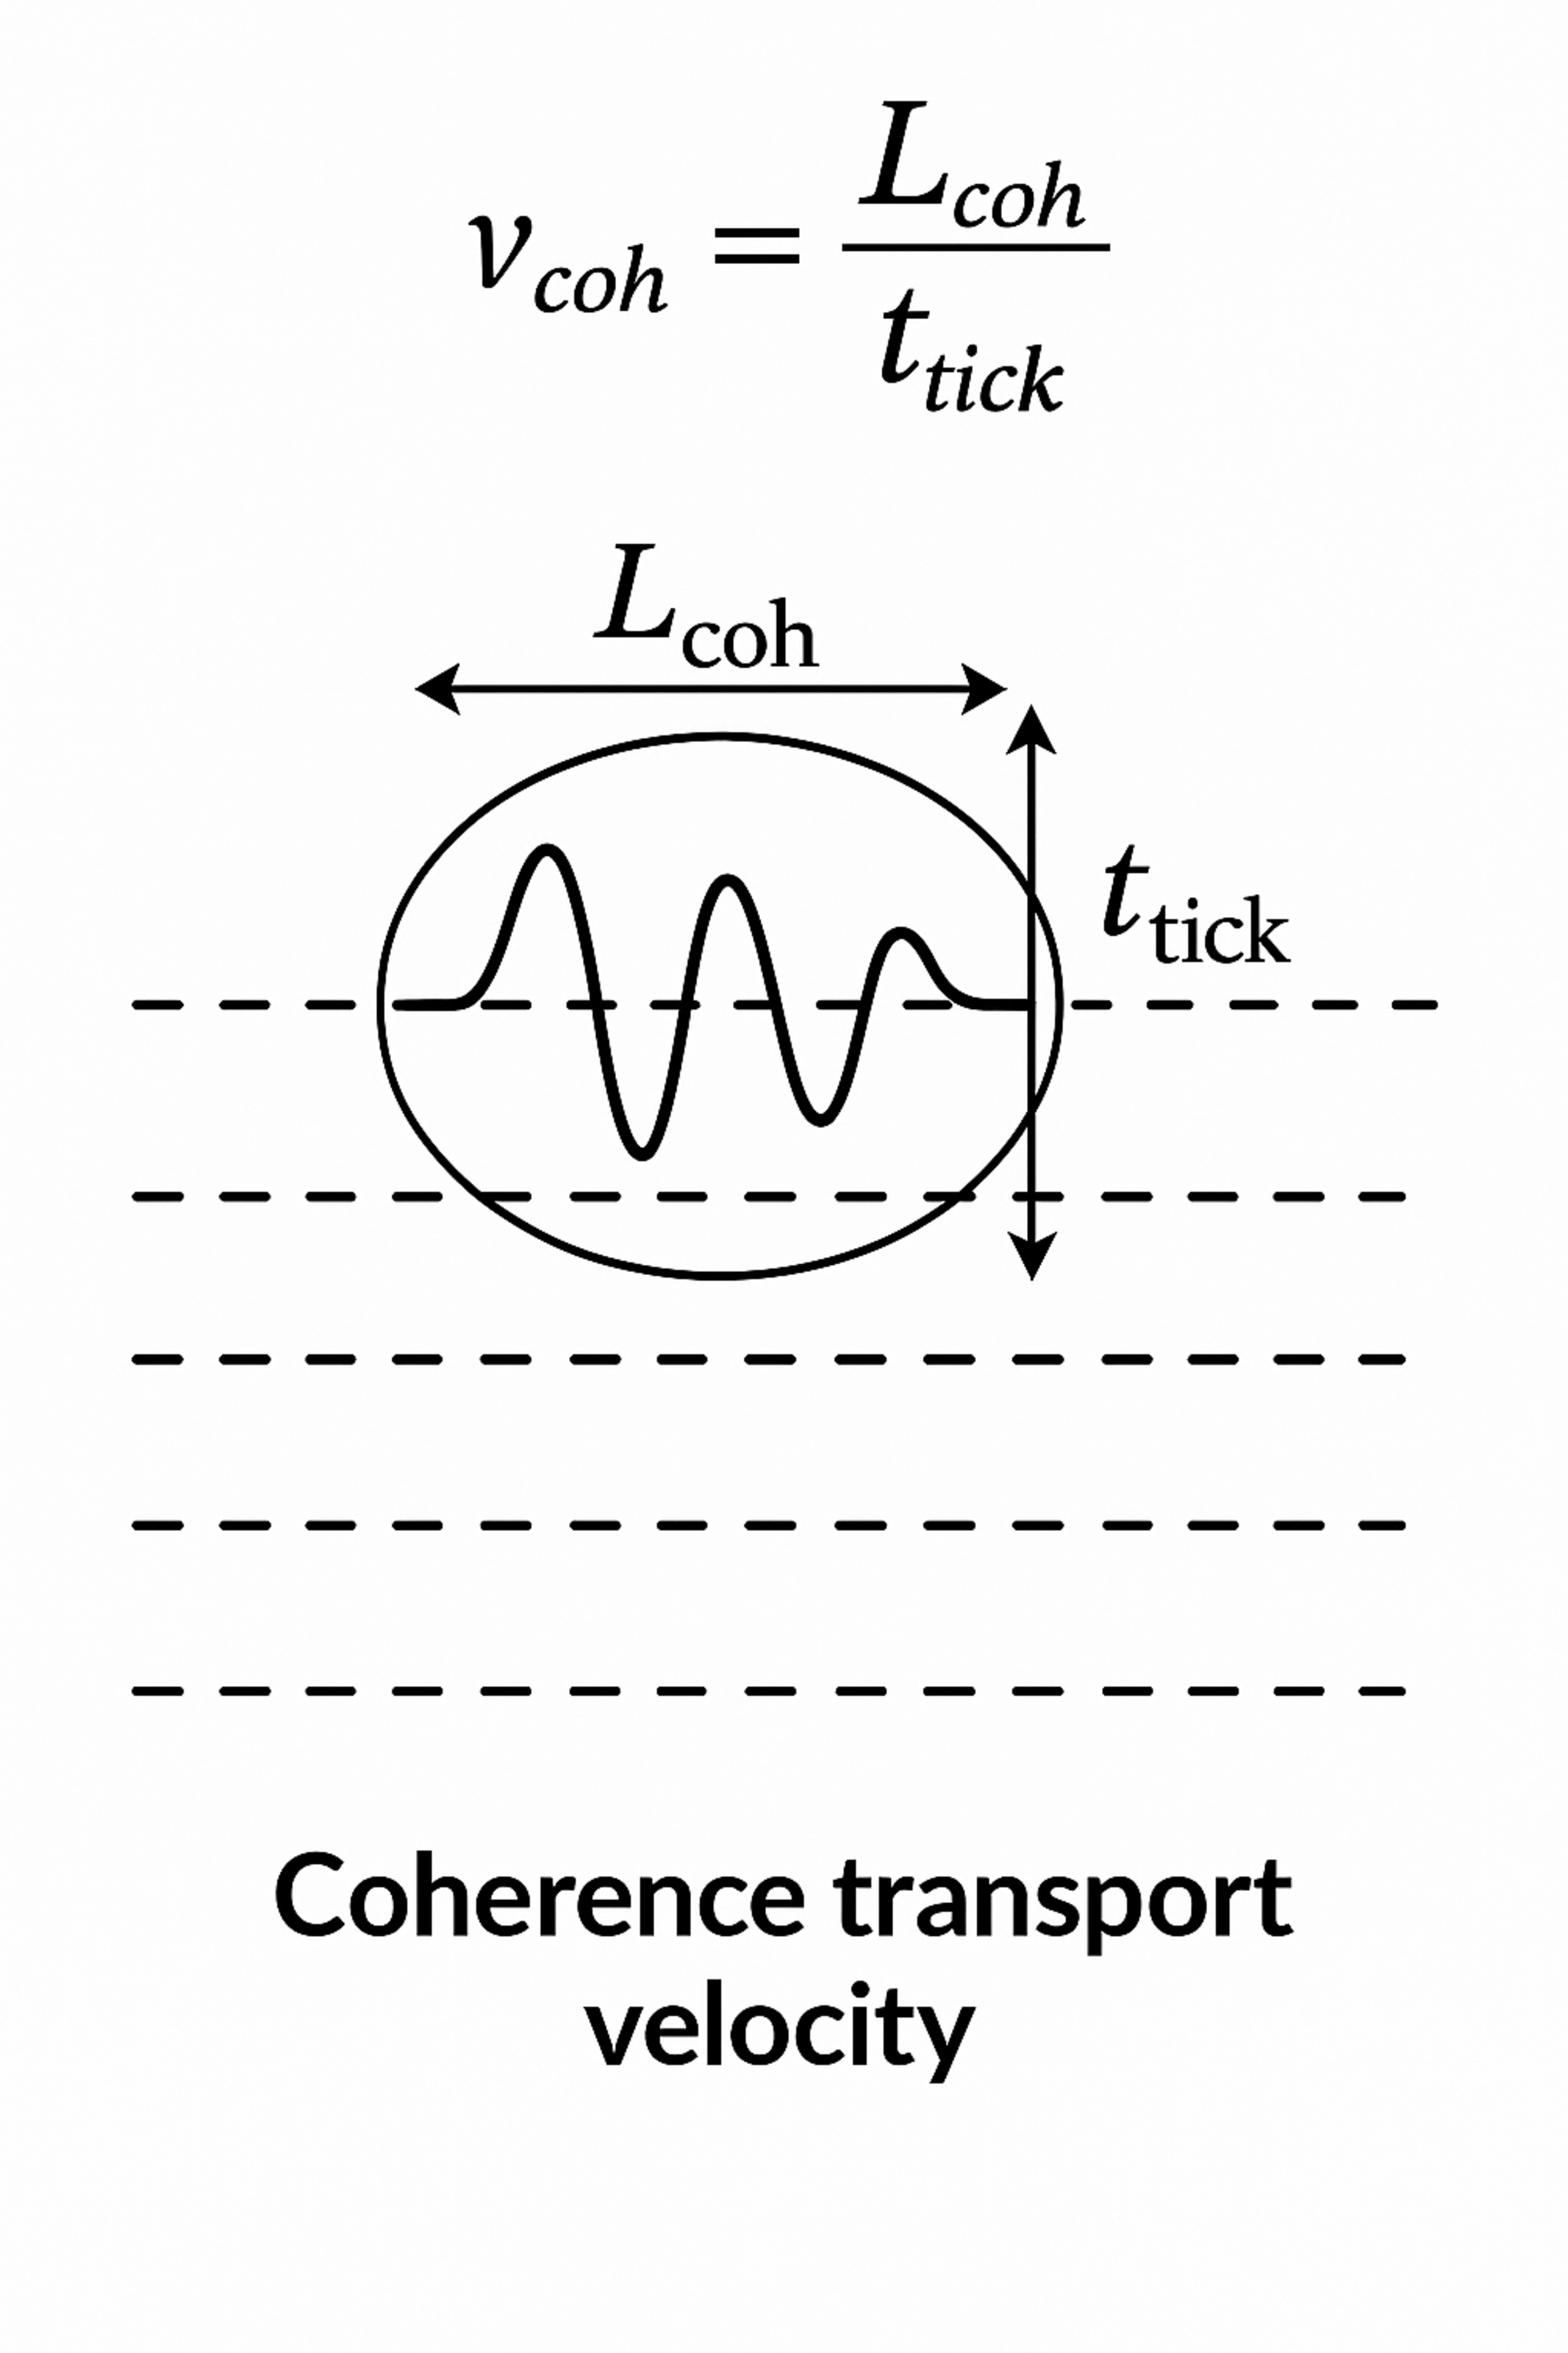
\includegraphics[width=0.6\textwidth]{figures/CTV.pdf}
    \caption{
    \textbf{Coherence Transport Velocity.} 
    In Quantum Substrate Dynamics (QSD), motion emerges explicitly as scalar-paced re-locking of coherent structures into adjacent substrate regions. The coherence transport velocity is defined as \( v_{\text{coh}} = \frac{L_{\text{coh}}}{t_{\text{tick}}} \), where the coherence envelope size \( L_{\text{coh}} \) is invariant under uniform motion, and \( t_{\text{tick}} \) is the scalar recovery interval. Velocity-induced increases in scalar coherence density within the fixed coherence envelope define a fundamental maximum mass--velocity threshold, beyond which scalar pacing constraints trigger structural collapse or scalar offload events.
    }
    \label{fig:coherence-transport-velocity}
\end{figure}

This reframing provides a physically transparent understanding of motion, inertia, and structural persistence. Stillness and uniform motion become structurally indistinguishable in tension-neutral substrates, differing only in scalar re-locking patterns. Motion explicitly arises when substrate gradients or scalar pacing conditions demand coherence reconfiguration, producing macroscopically measurable phenomena such as acceleration, inertial resistance, and scalar-mediated thermal emission.




%%%%%%%%%%%%%%%%%%%%%%%%%%%%%%%%%%%%%%%%%%%%%%%%%%%%%%%%
\subsection{Inertia as Scalar Reconfiguration Resistance}

In classical physics, inertia is treated as an intrinsic property of mass, represented as passive resistance to acceleration. Within the Quantum Substrate Dynamics (QSD) framework, inertia emerges instead as an active scalar resistance imposed by the substrate itself during the reconfiguration of coherent structure. Inertia is thus not a passive property carried by mass, but a dynamic structural response: the substrate’s scalar recovery lag when phase-coherent structures must re-lock under acceleration.

A mass-phase structure in QSD is defined by a stable configuration of scalar coherence locked within a substrate region bounded by the coherence envelope \( L_{\text{coh}} \). When acceleration occurs, the substrate is required to reconfigure the internal scalar coherence geometry into adjacent substrate regions at a rate that surpasses the local scalar pacing limit. Since the coherence envelope size \( L_{\text{coh}} \) remains invariant during uniform motion, increased velocity corresponds explicitly to an increase in the scalar coherence density within this fixed envelope, resulting in elevated substrate tension.

This elevated coherence density, when coupled with rapid directional or velocity changes, imposes significant scalar recovery demands. The scalar recovery process is constrained by the substrate’s minimum pacing interval—the Planck-scale tick \( t_{\text{tick}} \)—which defines the minimal causal time required for coherence re-locking. If an accelerating structure attempts to re-lock faster or differently than this scalar recovery interval permits, the substrate resists, imposing a scalar drag. Inertia, then, is explicitly this substrate resistance: the scalar recovery lag and energetic cost associated with phase geometry re-locking under acceleration.

Mathematically, inertial resistance in QSD can be expressed as a time-dependent scalar reconfiguration demand proportional to the local curvature and magnitude of the coherence phase gradient at the structure’s boundary:

\begin{equation}
    F_{\text{inertial}} \propto \kappa \frac{d}{dt} \nabla \theta(\vec{r}),
\end{equation}

where \(\nabla \theta(\vec{r})\) describes the local coherence-phase geometry at the boundary interface, and \(\kappa\) represents a substrate compliance constant characterizing the scalar recovery resistance. The inertial response thus arises structurally, scaling with the complexity and scalar tension associated with re-locking coherence boundaries at rates surpassing scalar pacing limits.

This interpretation clarifies the symmetry observed experimentally between acceleration and deceleration. Both phenomena represent directional changes in coherence re-locking, and in both cases, scalar coherence must be rapidly reconfigured, incurring similar structural and scalar recovery demands. From the substrate’s perspective, the direction of change is irrelevant; what matters is the scalar pacing constraint and the scalar tension incurred by rapid coherence re-locking. The inertial experience is therefore not the loss or gain of intrinsic momentum, but scalar response lag imposed by the substrate’s causal re-locking limitations.

By reframing inertia explicitly as scalar coherence reconfiguration resistance, QSD removes the need to regard mass as a primitive, fundamental property. Instead, mass is revealed structurally as the substrate's scalar recovery difficulty—the magnitude of scalar coherence density compression and boundary complexity determining how challenging it is to achieve rapid structural re-locking. This preserves all classical and relativistic experimental measurements of inertial mass, while providing a substrate-level explanation rooted directly in coherence geometry, scalar pacing, and structural causality.


%%%%%%%%%%%%%%%%%%%%%%%%%%%%%%%%%%%%%%%%%%
\subsection{Acceleration, Deceleration, and Momentum}

In the QSD framework, acceleration and deceleration are not fundamentally distinct phenomena; both represent scalar-paced changes in the reconfiguration of coherence structures. From the substrate’s perspective, uniform motion corresponds to a stable, tension-neutral scalar re-locking across sequential substrate regions, maintaining constant scalar coherence density within the fixed coherence envelope \(L_{\text{coh}}\). However, acceleration or deceleration impose new scalar pacing demands, requiring rapid or directionally modified re-locking and consequently altering the internal coherence-density distribution and phase geometry. Such reconfiguration introduces scalar recovery lag, boundary deformation, and measurable energetic consequences.

Momentum, in this interpretation, is not an intrinsic quantity carried passively by a mass, but a scalar-mediated structural alignment maintained by the substrate's ongoing commitment to coherence reconfiguration. It explicitly encodes how effectively a coherence structure is aligned to re-lock consistently and directionally across sequential causal intervals. Thus, momentum emerges as a structural memory of coherent scalar alignment rather than as a fundamental vector property.

Mathematically, momentum within the QSD framework can be explicitly defined as the integral of scalar coherence alignment over the coherence envelope:
\[
\vec{p}_{\text{QSD}} = \int_{\Omega} \rho(\vec{r}) \, \nabla \theta(\vec{r}) \, d^3r,
\]
where \(\rho(\vec{r})\) represents the local scalar coherence density, and \(\nabla \theta(\vec{r})\) describes the local phase-gradient geometry. This integral captures both directionality and the accumulated scalar coherence alignment, representing the substrate’s structural commitment to maintain a stable coherence path.

Importantly, the energetic consequences of momentum are not stored intrinsically within the moving structure itself, but rather reside explicitly in the substrate’s scalar coherence geometry and internal tension configuration. When motion changes abruptly—such as during a sudden stop or impact—the substrate’s ongoing coherence configuration is disrupted, leading to scalar rupture and immediate scalar offload into surrounding regions. The resulting energy release appears macroscopically as heat, vibration, or deformation, explicitly resolving the classical paradox of seemingly stored kinetic energy.

In QSD, acceleration, deceleration, and directional changes in velocity inherently involve scalar pacing demands. While uniform velocity does not alter the spatial size of the coherence envelope \(L_{\text{coh}}\), changes in velocity or direction require coherence reconfiguration at rates constrained by scalar pacing intervals (\(t_{\text{tick}}\)). Such reconfiguration elevates scalar tension and coherence density compression, which imposes structural and energetic costs measured as inertial resistance, scalar recovery lag, and thermal emission.

Thus, classical behaviors—including Newton’s laws and standard relativistic formulations—are preserved and naturally recovered as regime-specific outcomes of this scalar-paced coherence reconfiguration. However, the substrate-level interpretation replaces axiomatic assumptions of intrinsic mass or force with explicitly defined structural causality, coherence geometry, and scalar pacing logic.



%%%%%%%%%%%%%%%%%%%%%%%%%%%%%%%%%%%%%%%%%%
\subsection{Weight as Scalar Equilibrium Resistance}

In classical mechanics, weight is conventionally defined as a gravitational force acting on mass, \(W = mg\), where \(g\) represents the local gravitational field strength. While practically useful and predictive, this formulation describes what weight \emph{does}, but does not structurally explain what weight physically \emph{is}. In the Quantum Substrate Dynamics (QSD) framework, weight explicitly emerges as a structural consequence of the substrate’s scalar tension gradients and the resistance encountered when coherence re-locking into equilibrium configurations is structurally obstructed.

In QSD, gravity is not interpreted as an attractive force between masses, but rather as a gradient in scalar coherence tension within a conserved substrate. A mass-phase structure embedded in such a scalar tension gradient experiences a natural scalar-driven preference for re-locking its internal coherence geometry into regions of progressively lower tension. A free-falling object, for instance, continuously and freely re-locks along this gradient, experiencing no internal scalar deformation or resistance—thus it perceives no sensation of weight (see Figure~\ref{fig:weight-denied-relock}).

\begin{figure}[H]
    \centering
    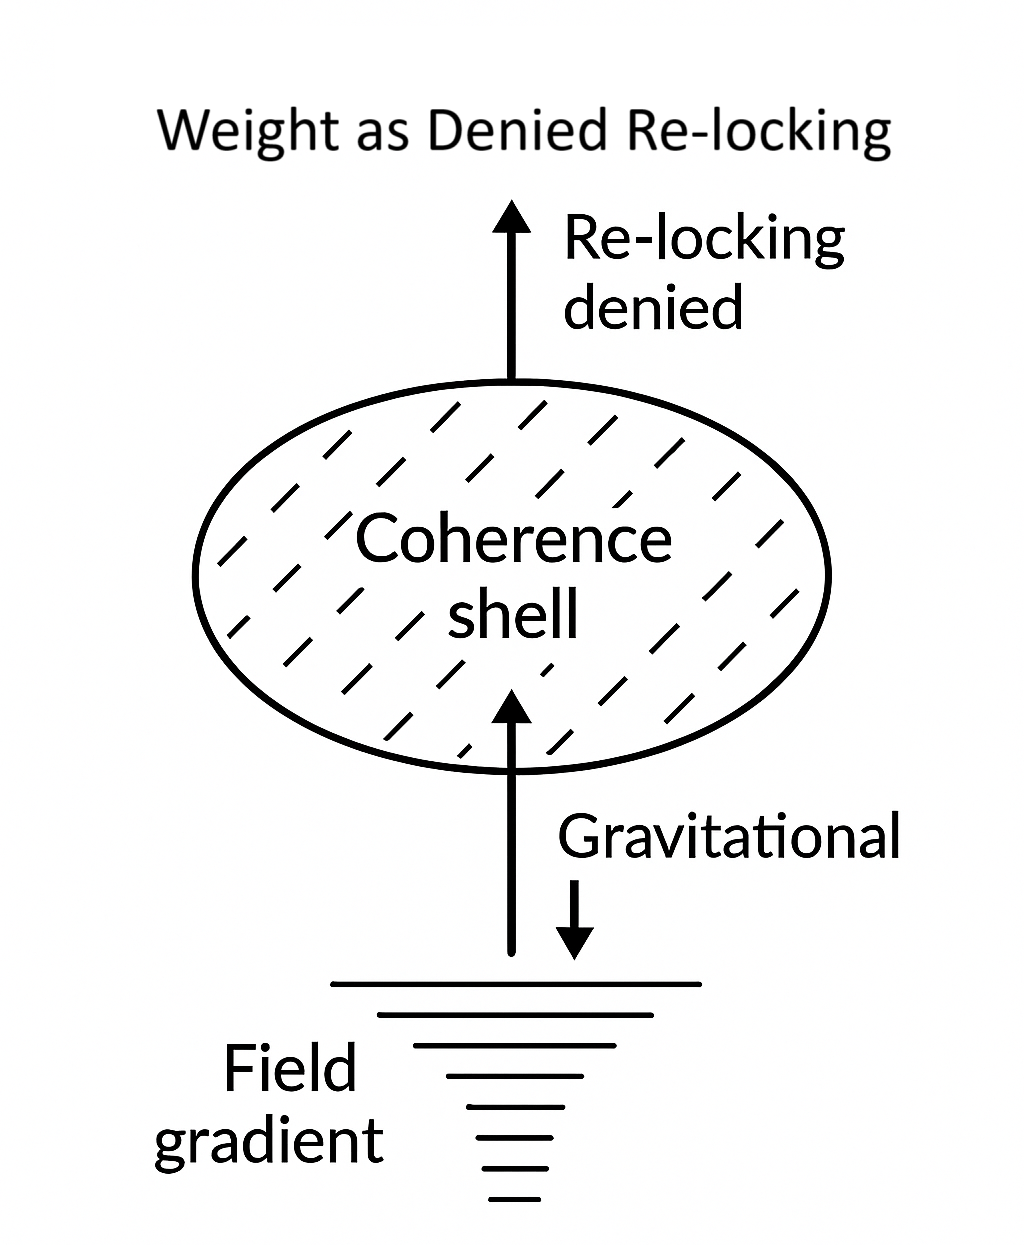
\includegraphics[width=0.5\textwidth]{figures/weight.png}
    \caption{
    \textbf{Weight as Denied Re-locking.}
    In Quantum Substrate Dynamics (QSD), weight is not a force acting across space but a structural resistance arising explicitly from denied scalar re-locking within a coherence gradient. A mass-phase coherence structure embedded in a gravitational scalar tension gradient attempts continuously to re-lock toward regions of lower substrate tension. When an external constraint—such as a surface—prevents this coherence realignment, the substrate imposes a scalar tension response in opposition to the denied re-locking direction. This scalar tension manifests macroscopically as weight, explicitly representing the local structural resistance due to substrate coherence denial rather than a fundamental gravitational attraction between masses.
    }
    \label{fig:weight-denied-relock}
\end{figure}

Weight explicitly appears in QSD only when coherence re-locking is structurally obstructed, such as when a structure is supported against a gravitational gradient by an external surface. Under these conditions, the substrate continuously attempts to re-lock the internal coherence geometry into lower-tension regions, but the re-locking is prevented by physical constraints. Consequently, the substrate experiences persistent scalar tension and imposes a scalar pushback that manifests macroscopically as the sensation of weight. Thus, weight emerges directly as a scalar resistance resulting from coherence re-lock denial across substrate gradients, not as a force transmitted through space.

This model naturally explains why free-falling objects appear weightless: their coherence structures re-lock continuously along the scalar tension gradient without substrate obstruction or scalar tension buildup. It similarly clarifies the microgravity experienced by orbiting astronauts, who remain continuously and coherently re-locking along gravitational gradients without scalar obstruction or resistance.

The scalar-gradient interpretation of weight also reframes gravitational interactions without invoking traditional attractive forces. A mass-phase structure creates substrate scalar tension gradients by its intrinsic coherence density and geometry. When another coherent structure enters such a gradient, it naturally tends toward re-locking into lower-tension substrate regions—not because of an intrinsic attractive force, but explicitly because reconfiguration into regions of lower scalar coherence tension minimizes deformation cost. Thus, gravitational motion is governed internally by coherence re-locking pathways and scalar tension differentials, rather than externally transmitted forces.

To explicitly formalize the substrate-level origin of weight, we define the scalar pushback integral:

\begin{equation}
    W = \int_{\Omega} \rho(\vec{r}) \, \nabla \Phi_{\text{coh}}(\vec{r}) \, d^3r,
\end{equation}

where \(\rho(\vec{r})\) is the local scalar coherence density, and \(\Phi_{\text{coh}}(\vec{r})\) describes the substrate's scalar tension potential and coherence alignment. This integral explicitly represents the scalar tension response of the substrate due to structurally denied re-locking toward equilibrium regions.

Under this substrate interpretation, Newton’s second law remains valid but is structurally reinterpreted. The classical equation \(F = ma\) becomes a regime-specific summary of scalar tension and coherence reconfiguration. Force arises explicitly from the substrate’s effort to resolve scalar tension when coherence realignment is obstructed or pacing constraints are imposed. Mass explicitly emerges as the scalar reconfiguration difficulty of structurally re-locking a given coherence configuration within pacing limits. Acceleration represents explicitly the increase in scalar pacing and reconfiguration demands.

Thus, QSD maintains compatibility with classical mechanics and relativistic dynamics while replacing gravitational attraction with explicit scalar tension gradients and substrate re-locking constraints. Weight becomes explicitly structural—emerging from the scalar coherence response to structurally obstructed realignment—rather than a fundamental force interaction.



%%%%%%%%%%%%%%%%%%%%%%%%%%%%%%%%%%%%%%%%%%
\subsection{Rotation and Angular Momentum}

Within classical mechanics, angular momentum is treated as a conserved property: the product of a body's moment of inertia and angular velocity. While successful in describing macroscopic behavior, classical theory does not structurally explain what angular momentum physically is or why rotating systems inherently resist directional change. Quantum Substrate Dynamics (QSD) provides a substrate-level interpretation in which angular momentum explicitly emerges as the substrate’s conserved scalar coherence curvature. In QSD, a rotating mass-phase structure produces a persistent deformation of coherence phase geometry within the substrate, and angular momentum explicitly represents the substrate’s scalar-structural commitment to maintaining this curved phase configuration.

Rotation differs fundamentally from linear scalar re-locking. Uniform linear motion within a tension-neutral substrate gradient involves coherent re-locking without persistent scalar curvature. In contrast, rotational motion inherently imposes a continuous coherence curvature requirement on the scalar substrate, demanding scalar re-locking into adjacent regions with systematically misaligned phase geometry. This continuously curved re-locking imposes structural strain, introducing substrate-level scalar tension and recovery lag that actively resists rapid directional changes.

The substrate explicitly stores this persistent deformation as a scalar torsional coherence pattern, representing a stable scalar-structural memory of angular configuration. Any attempt to change the rotation axis or angular velocity thus imposes additional scalar recovery demands, as the substrate must actively restructure coherence geometry, a process that is structurally and energetically costly. Gyroscopic resistance explicitly emerges as the substrate’s scalar commitment to conserving angular coherence curvature against directional perturbation.

Angular momentum, in QSD, is therefore not an intrinsic vector carried passively by mass, but a substrate-embedded scalar curvature integral defined explicitly by coherence geometry and phase gradient:

\[
\vec{L}_{\text{QSD}} = \int_{\Omega} \rho(\vec{r})\left(\vec{r}\times\nabla\theta(\vec{r})\right)\,d^3r,
\]

where \(\rho(\vec{r})\) represents the local scalar coherence density, and \(\nabla\theta(\vec{r})\) encodes the local phase gradient tangent to the coherence structure’s curved scalar re-locking path. Thus, angular momentum explicitly quantifies the scalar coherence curvature structurally sustained by the substrate, rather than merely the classical kinematic property of mass rotation.

Rotational motion explicitly introduces scalar recovery lag into the substrate dynamics. Persistent curved re-locking cycles cannot occur instantly; scalar tension accumulates within the substrate, requiring subsequent scalar offload as thermal emission or coherence jitter at coherence boundaries. Even uniform rotation, absent classical friction, leads to measurable thermal dissipation. More rapid directional changes—such as those involved in tilting or accelerating gyroscopic systems—explicitly increase this scalar recovery lag, accelerating offload processes, producing spin-down, and increasing observable heating. Such scalar-mediated thermal signatures cannot be explained adequately by classical friction or damping.

The scalar offload resulting explicitly from persistent rotational curvature can be modeled structurally as a scalar offload power function:

\[
P_{\text{offload}}(t) = \gamma \cdot \frac{\Delta E_{\text{torsion}}}{\tau},
\]

where \(\Delta E_{\text{torsion}}\) represents the accumulated scalar coherence strain energy due to persistent torsional curvature within the coherence geometry, \(\tau\) defines the scalar recovery timescale, and \(\gamma\) is a coupling constant relating scalar coherence tension explicitly to measurable thermal or radiative emission. This substrate-based formulation explicitly predicts scalar-driven thermal emission correlated with rotational coherence curvature and scalar pacing lag, even in isolated systems.

In QSD, angular momentum explicitly emerges as a structurally conserved but energetically costly scalar coherence curvature phenomenon. A rotating coherence structure explicitly invests scalar curvature memory within the substrate, structurally constraining directional changes and imposing scalar recovery demands. This substrate-based reframing explicitly explains gyroscopic resistance, spin decay, inertial rigidity, and angular momentum conservation structurally—from first principles—without invoking mass as fundamental or relying on axiomatic conservation laws (see Figure~\ref{fig:inertial-resistance}).

\begin{figure}[H]
    \centering
    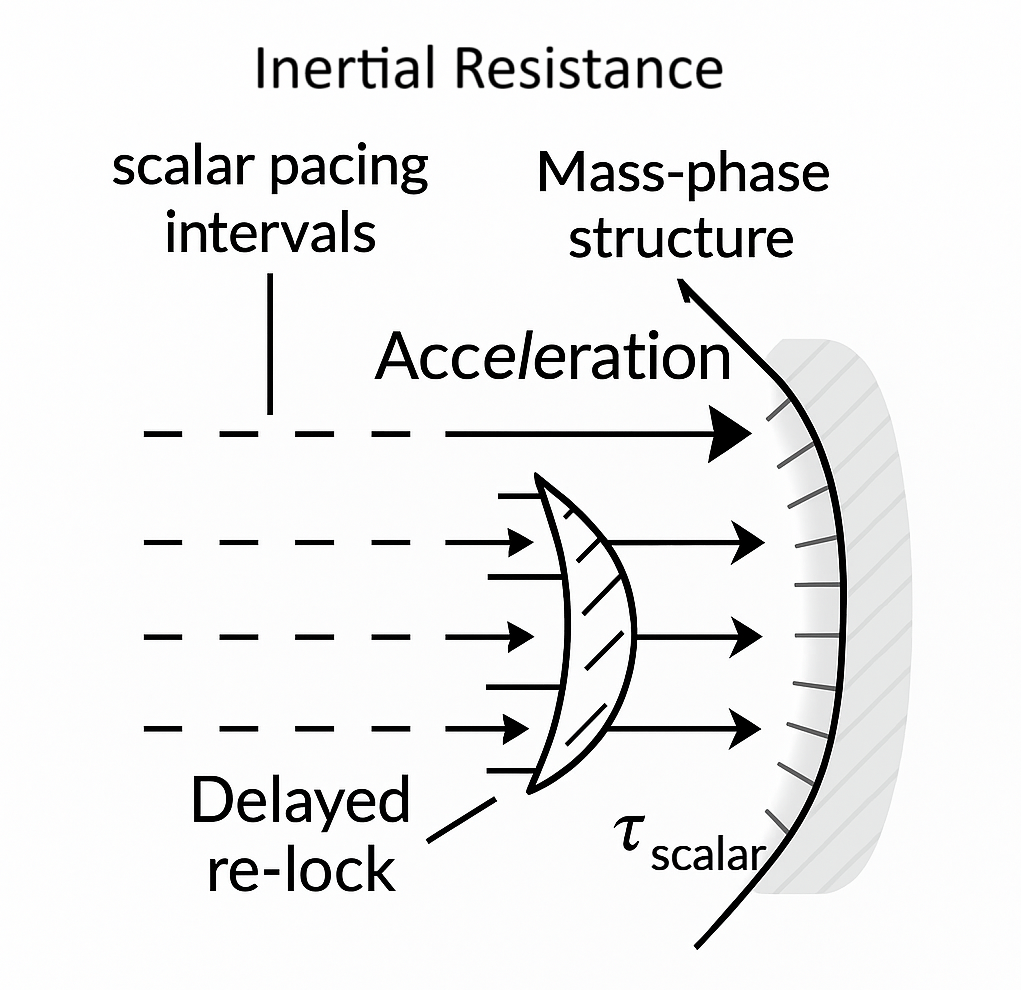
\includegraphics[width=0.6\textwidth]{figures/inertia.png}
    \caption{
    \textbf{Inertial Resistance and Scalar Pacing.}
    In Quantum Substrate Dynamics (QSD), inertial resistance arises explicitly from scalar pacing constraints imposed during the structural re-locking of a coherence boundary. As a coherence structure undergoes rotational or directional acceleration, its scalar re-locking into the substrate becomes increasingly desynchronized, resulting explicitly in scalar coherence lag or deformation. This scalar recovery delay (\(\tau_{\text{scalar}}\)) explicitly defines the scalar pacing-limited resistance experienced macroscopically as inertia. The substrate explicitly enforces a minimal scalar pacing interval between re-locking events, making inertia explicitly a scalar coherence pacing response rather than an intrinsic property of mass.
    }
    \label{fig:inertial-resistance}
\end{figure}

%%%%%%%%%%%%%%%%%%%%%%%%%%%%%%%%%%%%%%%%%%
\subsection{Energy and Motion}

In classical physics, energy is treated as a transferable, conserved quantity stored within physical objects, manifesting explicitly as kinetic or potential energy forms. Within the Quantum Substrate Dynamics (QSD) framework, energy is structurally reinterpreted not as a quantity stored inherently within objects, but explicitly as the scalar-mediated procedural effort required to sustain or alter phase-coherent structures within the substrate. Energetic phenomena explicitly emerge when coherence boundaries undergo deformation, scalar tension, displacement, or scalar-paced re-locking transitions.

Uniform scalar re-locking under tension-neutral substrate gradients—corresponding explicitly to uniform motion—does not inherently carry or expend energy. Such motion occurs explicitly via substrate coherence re-locking that is structurally continuous, energetically silent, and scalar-tension neutral. Energy expenditures explicitly arise only when motion undergoes scalar-pacing deviations: acceleration, deceleration, directional changes, rotation, or coherence misalignment, each requiring active scalar substrate reconfiguration effort.

Kinetic energy, therefore, is not something intrinsically "possessed" by moving coherence structures. Rather, kinetic energy explicitly represents the scalar substrate's effort to structurally maintain coherence geometry and scalar alignment under motion conditions requiring substrate deformation or scalar pacing demands. Potential energy is explicitly reframed as the scalar substrate's readiness or structural tendency to re-lock coherence geometry into lower-tension equilibrium configurations—such as when a coherence structure is positioned within or constrained above a gravitational substrate tension gradient.

Thermal energy emerges explicitly when scalar re-locking fails to occur cleanly and coherently within scalar pacing constraints. Under scalar reconfiguration demands—such as repeated structural deformation, acceleration cycles, or persistent rotational curvature—the scalar substrate accumulates coherence tension and pacing lag, saturating scalar memory. Scalar offload events explicitly release this accumulated tension, dissipating it structurally as low-scale coherence jitter or scalar thermal offload. Macroscopically, this scalar offload explicitly appears as measurable heat, clarifying why mechanical systems warm under repeated structural deformation—even in frictionless, isolated environments.

The scalar offload power equation introduced here,
\[
P_{\text{offload}}(t) = \gamma \cdot \frac{\Delta E_{\text{torsion}}}{\tau},
\]
offers a clear candidate for simulation and future quantitative modeling. Estimating thermal output in rotating systems will require approximating the scalar curvature strain energy (\( \Delta E_{\text{torsion}} \)), the scalar recovery timescale (\( \tau \)), and the substrate-specific coupling constant (\( \gamma \)) for a given configuration. While precise values remain subject to further modeling, even approximate simulations of this offload behavior could provide falsifiable predictions—particularly in high-precision gyroscopic systems or isolated rotors operating under vacuum conditions. These efforts are deferred to future work but represent an actionable path toward experimental validation and substrate parameter refinement.


Within QSD, energy conservation is structurally explicit. Energy explicitly emerges from the substrate's scalar effort to maintain and realign coherence geometry across causal intervals, substrate gradients, and scalar pacing constraints. What classical physics interprets as conserved energy explicitly arises as the scalar-mediated redistribution and structural resolution of scalar tension and recovery effort. When a coherence structure transitions to rest, its apparent "lost" kinetic energy explicitly undergoes scalar offload into the substrate, structurally reconfiguring scalar coherence geometry and incurring scalar recovery delay. This explicit scalar offload process provides a physically transparent mechanism for energy transformation and dissipation, without resorting to abstract fields or hidden energy reservoirs.

QSD explicitly reframes energy as an emergent scalar-mediated behavior governed by substrate coherence geometry and scalar pacing management. Uniform motion, explicitly characterized by tension-neutral scalar re-locking, is energetically neutral unless scalar substrate conditions explicitly require structural reconfiguration or scalar coherence geometry deformation. Only when substrate geometry or scalar pacing explicitly demands active coherence realignment does scalar tension accrue, resulting explicitly in energy expenditure. Thus, energy explicitly represents the scalar-mediated cost structurally paid by the substrate to maintain and realign coherence geometry—not something stored inherently within moving structures.



%%%%%%%%%%%%%%%%%%%%%%%%%%%%%%%%%%%%%%%%%%
\subsection{Compatibility with Classical Physics}

The Quantum Substrate Dynamics (QSD) framework explicitly reframes motion, inertia, momentum, and energy as emergent phenomena structurally arising from scalar coherence dynamics and substrate pacing, rather than as primitive or axiomatic concepts. Despite this foundational shift, QSD remains explicitly and fully compatible with classical and relativistic physics within their respective predictive domains. Classical equations of motion, Newtonian mechanics, and Einstein's relativistic kinematics emerge naturally as regime-specific approximations of scalar substrate response under suitable limiting conditions.

QSD explicitly preserves classical conservation laws, including energy, linear momentum, and angular momentum, but structurally reinterprets them explicitly as substrate-mediated coherence geometry and scalar tension symmetry. Newton’s second law, \(F = ma\), is explicitly recovered as a large-scale summary of scalar substrate resistance arising from scalar coherence deformation and re-locking demands. Force explicitly arises as scalar tension resulting from structural reconfiguration constraints, acceleration explicitly reflects scalar pacing demand for rapid coherence re-locking, and mass explicitly emerges structurally from scalar coherence-density compression and scalar recovery resistance.

Inertial reference frame equivalence, as formulated explicitly by Einstein, emerges naturally in QSD from scalar neutrality and scalar re-locking symmetry within tension-balanced substrate regions. Lorentz invariance is explicitly upheld through the scalar pacing limit defined by the substrate's minimal causal recovery interval (\(t_{\text{tick}}\)), explicitly ensuring that no scalar coherence structure can re-lock faster than the substrate’s scalar recovery speed (\(c_s\)). Thus, QSD explicitly maintains relativistic causality and maximum propagation constraints structurally and explicitly.

Classical paradoxes and interpretive ambiguities—such as the equivalence of rest and uniform velocity, the source of inertial resistance, or energetic consequences of collisions—are explicitly resolved structurally and explicitly within QSD, without altering their experimentally confirmed predictions. Uniform motion explicitly corresponds to structurally tension-neutral scalar re-locking, and inertial resistance explicitly arises structurally from scalar pacing lag under accelerated coherence reconfiguration. Energetic outcomes explicitly result from scalar coherence reconfiguration effort and scalar offload during substrate-mediated scalar recovery lag, explicitly replacing the abstract concept of intrinsic energy storage with explicit substrate geometry and scalar coherence mechanisms.

The general relativistic interpretation of gravity as geometric spacetime curvature explicitly finds a coherent structural analog in QSD. Gravitational phenomena explicitly emerge from scalar coherence tension gradients within the substrate, explicitly providing structural explanations for observed gravitational behaviors such as orbital dynamics, free fall, and gravitational time dilation. Scalar coherence geometry explicitly replaces abstract geometric postulation, explicitly producing gravitational predictions fully compatible with classical general relativity while offering structural substrate-level clarity and explicit scalar causality.

Crucially, QSD explicitly does not negate classical, relativistic, or quantum theories; instead, it structurally grounds and explicitly extends their conceptual foundations. Classical and relativistic behaviors explicitly emerge explicitly as substrate-level scalar coherence responses in appropriate scalar and structural limits. Quantities traditionally treated as axiomatic or abstract—such as mass, inertia, force, and energy—are explicitly reinterpreted structurally as scalar-mediated coherence dynamics and explicitly derived scalar coherence geometry. Thus, QSD explicitly preserves continuity and explicit compatibility with established theoretical predictions, explicitly extending their interpretive and structural foundations through explicitly causally coherent, explicitly falsifiable scalar substrate mechanisms.



%%%%%%%%%%%%%%%%%%%%%%%%%%%%%%%%%%%%%%%%%%
\subsection{Reframing Motion as Emergent Coherence Dynamics}

The results presented in this work invite a fundamental reconsideration of how motion, inertia, and momentum are understood—not as primitive, axiomatic quantities, but as explicitly emergent behaviors arising from scalar coherence structures embedded within a conserved substrate. Quantum Substrate Dynamics (QSD) provides a physically grounded structural mechanism for phenomena traditionally treated as intrinsic: inertia explicitly emerges as scalar coherence reconfiguration resistance, motion explicitly becomes scalar-paced re-locking of coherence geometry, and momentum explicitly reflects the substrate's ongoing structural commitment to preserving scalar coherence alignment along a trajectory.

This structural reframing does not discard or challenge existing classical or relativistic physics; rather, it explicitly reveals the deeper scalar substrate continuity underpinning their successful predictive frameworks. Classical mechanics remains explicitly valid as large-scale, regime-specific approximations of scalar coherence dynamics, while relativistic constraints explicitly emerge from the scalar recovery and pacing limits inherent in the substrate. The explicit strength of the QSD framework lies precisely in its capacity to provide causal, scalar-substrate explanations for phenomena previously considered axiomatic or abstract—explicitly including inertial resistance, the structural indistinguishability of rest and uniform motion, and the inherent scalar-pacing symmetry between acceleration and deceleration.

Moreover, this structural interpretation explicitly provides substrate-based explanations for observable thermal phenomena and apparent energy dissipation in rotating systems. The scalar coherence curvature inherent in rotational motion explicitly introduces persistent scalar recovery lag and scalar tension accumulation, structurally resulting in measurable thermal offload, even in idealized frictionless or vacuum conditions. Scalar offload explicitly explains why rotating systems exhibit measurable heating after directional changes—such thermal signatures explicitly emerge structurally from incomplete scalar coherence recovery and substrate tension saturation, scaling explicitly with angular strain magnitude and scalar pacing constraints.

At the broadest level, placing scalar coherence explicitly at the structural foundation of all motion leads to an explicit reinterpretation of mass and energy not as intrinsic properties but as explicitly emergent scalar-substrate outcomes. Mass explicitly emerges structurally as the scalar substrate's coherence re-locking difficulty and scalar recovery resistance, while energy explicitly emerges structurally as scalar coherence tension management and substrate recovery effort. This substrate-level reinterpretation has profound implications explicitly beyond classical dynamics, extending explicitly into quantum behavior, field interactions, and even explicit models of spacetime geometry at the most fundamental scalar coherence level.

Thus, this work explicitly advances toward a physically transparent substrate-based interpretation of motion, explicitly rooted not in abstract concepts of force or intrinsic mass, but explicitly in scalar coherence geometry and substrate causal logic. Such structural clarity explicitly enables novel experimental pathways explicitly including scalar-based inertial sensing, post-rotation thermal signature characterization, and explicit coherence-guided transport mechanisms. The goal explicitly is not to reject or displace established physics, but explicitly to structurally ground and unify its explanatory foundations within a single conserved scalar coherence substrate—where explicitly motion, inertia, and structure are explicitly inseparable scalar-mediated aspects of a singular conserved reality.



%%%%%%%%%%%%%%%%%%%%%%%%%%%%%%%%%%%%%%%%%%%
\section{Conclusion}
%%%%%%%%%%%%%%%%%%%%%%%%%%%%%%%%%%%%%%%%%%%
This work has presented a structural derivation of motion, inertia, and momentum under the framework of General Substrate Theory (GST), using the dynamic principles of Quantum Substrate Dynamics (QSD). By modeling mass-phase structures as phase-stable coherence knots embedded in a conserved substrate, we have shown that motion is not geometric traversal, but a sequence of scalar-paced re-locking events governed by a minimum causal interval—the Planck-scale tick. Inertia emerges from the substrate’s resistance to accelerated reconfiguration, momentum reflects the coherence already committed to a re-locking path, and weight arises from denied alignment with a scalar gradient.

Rotational motion was shown to impose persistent curvature strain on the substrate, producing irreversible scalar offload and thermal dissipation—even in the absence of classical friction. Angular momentum is reinterpreted as conserved phase curvature, and gyroscopic resistance emerges as the substrate’s structural commitment to preserving coherence geometry under rotation. These effects are not appended to physics—they are revealed as deeper substrate responses beneath familiar macroscopic and quantum behaviors.

Classical laws are preserved, but reinterpreted as emergent approximations of coherence structure evolving under causal constraint. Motion, stillness, and resistance are no longer distinct categories—they are continuous expressions of scalar re-locking dynamics. This work reframes Newtonian and relativistic behaviors as surface-level expressions of a deeper substrate ontology in which coherence, timing, and structural commitment define all observable dynamics.

This reinterpretation enables new approaches to modeling mechanical systems, inertial asymmetry, and thermally coupled motion from first principles. It provides a physical explanation for post-rotation heating, scalar recovery lag, and memory-linked inertial resistance. It also lays the groundwork for future investigations into coherence-bound transport, substrate-sensing technologies, and scalar-informed quantum behavior. By rooting motion in Planck-paced reconfiguration, General Substrate Theory offers a causally coherent and physically testable foundation—one in which motion, inertia, and structure are inseparable consequences of conserved coherence in an active substrate.

%While this work introduces the structural and causal foundations of QSD, future work will aim to establish correspondence with classical and quantum formalisms in appropriate limiting cases. In particular, Newtonian dynamics, relativistic kinematics, and quantum behaviors are expected to emerge from substrate coherence reconfiguration under tension-neutral, low-curvature regimes. These reductions will further support continuity with existing physics while maintaining the causal substrate mechanisms unique to QSD.


%%%%%%%%%%%%%%%%%%%%%%%%%%%%%%%%%%%%%%%%%%
\vspace{6pt} 

%%%%%%%%%%%%%%%%%%%%%%%%%%%%%%%%%%%%%%%%%%
%% optional
%\supplementary{The following supporting information can be downloaded at:  \linksupplementary{s1}, Figure S1: title; Table S1: title; Video S1: title.}

% Only for journal Methods and Protocols:
% If you wish to submit a video article, please do so with any other supplementary material.
% \supplementary{The following supporting information can be downloaded at: \linksupplementary{s1}, Figure S1: title; Table S1: title; Video S1: title. A supporting video article is available at doi: link.}

% Only used for preprtints:
% \supplementary{The following supporting information can be downloaded at the website of this paper posted on \href{https://www.preprints.org/}{Preprints.org}.}

% Only for journal Hardware:
% If you wish to submit a video article, please do so with any other supplementary material.
% \supplementary{The following supporting information can be downloaded at: \linksupplementary{s1}, Figure S1: title; Table S1: title; Video S1: title.\vspace{6pt}\\
%\begin{tabularx}{\textwidth}{lll}
%\toprule
%\textbf{Name} & \textbf{Type} & \textbf{Description} \\
%\midrule
%S1 & Python script (.py) & Script of python source code used in XX \\
%S2 & Text (.txt) & Script of modelling code used to make Figure X \\
%S3 & Text (.txt) & Raw data from experiment X \\
%S4 & Video (.mp4) & Video demonstrating the hardware in use \\
%... & ... & ... \\
%\bottomrule
%\end{tabularx}
%}

\section*{Statements and Declarations}
\subsection*{Funding}  
The author received no financial support for the research, authorship, or publication of this article.
The author has no relevant financial or non-financial interests to disclose.

\subsection*{Competing Interests}  
The author declares no competing interests.

\subsection*{Author Contributions}  
The author solely conceived, developed, and wrote the manuscript, including all theoretical content, references, and formatting.

\subsection*{Data Availability}  
No datasets were generated or analyzed during the current study. All references are publicly available.

\subsection*{Ethical Approval}  
Not applicable.


%%%%%%%%%%%%%%%%%%%%%%%%%%%%%%%%%%%%%%%%%%
%% Optional

%% Only for journal Encyclopedia
%\entrylink{The Link to this entry published on the encyclopedia platform.}

\abbreviations{Abbreviations}{
The following abbreviations are used in this manuscript:
\\

\noindent
\begin{tabular}{@{}ll}
QSD   & Quantum Substrate Dynamics \\
\( c_s \) & Scalar coherence recovery speed (temporal mode) \\
\( c_t \) & Transverse coherence propagation speed (spatial mode) \\
\( L_0 \) & Baseline coherence length at rest \\
\( L_{\text{coh}}(r) \) & Curvature-stretched coherence support length \\
\( v \) & Apparent velocity relative to substrate \\
\( v_{\text{coh}} \) & Coherence transport velocity \( = \frac{L_{\text{coh}}}{t_{\text{tick}}} \) \\
\( t_{\text{tick}} \) & Local scalar recovery interval (effective time tick) \\
\( t_0 \) & Tick duration at rest (baseline tick) \\
\( \kappa \) & Substrate compliance constant (resistance to boundary deformation) \\
\( \theta(\vec{r}) \) & Local coherence phase at position \( \vec{r} \) \\
\( \rho(\vec{r}) \) & Coherence density distribution \\
\( F_{\text{inertial}} \) & Inertial response force under reconfiguration stress \\
\( P_{\text{offload}}(t) \) & Scalar thermal offload power over time \\
\( \Delta E_{\text{torsion}} \) & Accumulated torsional energy due to rotational strain \\
\( \tau \) & Scalar recovery lag timescale \\
\( \gamma \) & Lorentz factor (compatible structural form) \\
GPS  & Global Positioning System \\
SR   & Special Relativity \\
GR   & General Relativity \\
\end{tabular}

}



%%%%%%%%%%%%%%%%%%%%%%%%%%%%%%%%%%%%%%%%%%
%% Optional
\appendixtitles{no} % Leave argument "no" if all appendix headings stay EMPTY (then no dot is printed after "Appendix A"). If the appendix sections contain a heading then change the argument to "yes".
\appendixstart
\appendix
%%%%%%%%%%%%%%%%%%%%%%%%%%%%%%%%%%%%%%%%%%%%%%%
\section[\appendixname~\thesection]{}
\subsection[\appendixname~\thesubsection]{Canonical QSD Motion Equations}
%%%%%%%%%%%%%%%%%%%%%%%%%%%%%%%%%%%%%%%%%%%%%%
The following expressions summarize the core structural relationships introduced in this paper. Each equation explicitly reflects a substrate-level mechanism associated with motion, inertia, momentum, thermal offload, or gravitational resistance, redefined within the Quantum Substrate Dynamics (QSD) framework.

\subsubsection{Inertial Resistance}
Inertia explicitly arises as scalar resistance when coherence re-locking must occur faster or in a more structurally complex manner than the substrate’s causal pacing allows:
\begin{equation}
    F_{\text{inertial}} \propto \kappa \cdot \frac{d}{dt} \nabla \theta(\vec{r}),
\end{equation}
where \(\kappa\) is the substrate compliance constant, characterizing explicit scalar coherence resistance, and \(\nabla \theta(\vec{r})\) describes explicitly the local phase geometry gradient at the coherence boundary.

\subsubsection{Momentum as Coherence Path Commitment}
Momentum explicitly represents the scalar coherence alignment maintained structurally across sequential substrate regions by a mass-phase coherence structure:
\begin{equation}
    \vec{p}_{\text{QSD}} = \int_{\Omega} \rho(\vec{r}) \, \nabla \theta(\vec{r}) \, d^3r,
\end{equation}
where \(\rho(\vec{r})\) is explicitly the local scalar coherence density, and \(\nabla \theta(\vec{r})\) explicitly encodes the local scalar coherence geometry describing structural alignment and substrate commitment to maintaining a scalar coherence path.

\subsubsection{Rotational Offload Power}
Rotational motion explicitly introduces scalar coherence curvature, resulting explicitly in persistent scalar recovery lag and measurable scalar thermal offload:
\begin{equation}
    P_{\text{offload}}(t) = \gamma \cdot \frac{\Delta E_{\text{torsion}}}{\tau},
\end{equation}
where \(\Delta E_{\text{torsion}}\) explicitly represents the accumulated scalar coherence strain energy due to rotational curvature, \(\tau\) explicitly defines the scalar coherence recovery timescale, and \(\gamma\) explicitly relates scalar coherence tension explicitly to measurable thermal scalar offload rate.

\subsubsection{Weight from Gradient Tension}
Weight explicitly emerges structurally as scalar substrate pushback when scalar coherence re-locking into lower-tension substrate regions is structurally obstructed:
\begin{equation}
    W = \int_{\Omega} \rho(\vec{r}) \cdot \nabla \Phi_{\text{coh}}(\vec{r}) \, d^3r,
\end{equation}
where \(\rho(\vec{r})\) explicitly represents the scalar coherence density, and \(\Phi_{\text{coh}}(\vec{r})\) explicitly defines the scalar coherence tension potential of the substrate gradient.

\subsubsection{Coherence Transport Velocity}
The explicit velocity of motion within QSD is governed structurally by the scalar pacing limit of coherence re-locking, rather than by geometric traversal. The coherence envelope size (\(L_{\text{coh}}\)) explicitly remains invariant under uniform velocity, with velocity-induced effects explicitly appearing as scalar coherence density compression within this fixed envelope:
\begin{equation}
    v_{\text{coh}} = \frac{L_{\text{coh}}}{t_{\text{tick}}},
\end{equation}
where \(L_{\text{coh}}\) explicitly defines the invariant coherence envelope length, and \(t_{\text{tick}}\) explicitly defines the local scalar recovery pacing interval. Velocity explicitly emerges structurally as scalar pacing-dependent coherence re-lock rate, constrained explicitly by scalar coherence density and causal pacing limits, and explicitly independent of direct geometric deformation of the coherence envelope size.

\vspace{1em}

These explicitly defined expressions serve explicitly as the foundational scalar-substrate mechanics for motion, inertia, momentum, thermal offload, and gravitational phenomena within the Quantum Substrate Dynamics (QSD) framework. Each explicitly replaces classical kinematic assumptions explicitly with structurally grounded scalar coherence geometry, scalar pacing constraints, and explicit substrate-level causal conservation principles.



%%%%%%%%%%%%%%%%%%%%%%%%%%%%%%%%%%%%%%%%%%%%%%

%%%%%%%%%%%%%%%%%%%%%%%%%%%%%%%%%%%%%%
%\subsubsection{SUB A}
%%%%%%%%%%%%%%%%%%%%%%%%%%%%%%%%%%%%%%

%%%%%%%%%%%%%%%%%%%%%%%%%%%%%%%%%%%%%%%%%%%%%%%
%\section[\appendixname~\thesection]{}
%\subsection[\appendixname~\thesubsection]{APP B}
%%%%%%%%%%%%%%%%%%%%%%%%%%%%%%%%%%%%%%%%%%%%%%%

%\subsubsection{SUB B}

%%%%%%%%%%%%%%%%%%%%%%%%%%%%%%%%%%%%%%%%%%
\isPreprints{}{% This command is only used for ``preprints''.
\begin{adjustwidth}{-\extralength}{0cm}
} % If the paper is ``preprints'', please uncomment this parenthesis.
%\printendnotes[custom] % Un-comment to print a list of endnotes

\reftitle{References}

% Please provide either the correct journal abbreviation (e.g. according to the “List of Title Word Abbreviations” http://www.issn.org/services/online-services/access-to-the-ltwa/) or the full name of the journal.
% Citations and References in Supplementary files are permitted provided that they also appear in the reference list here. 

%=====================================
% References, variant A: external bibliography
%=====================================
% \bibliography{your_external_BibTeX_file}

%=====================================
% References, variant B: internal bibliography
%=====================================

% ACS format
\isAPAandChicago{}{%
\begin{thebibliography}{999}
% Reference 
\bibitem{bush2025}
\textbf{Preprint.} Bush, M. (2025). Quantum Substrate Dynamics (QSD): A Relativistic Field Model of Emergent Mass, Inertia and Gravity. \textit{Preprints}, 2025060988. \url{https://doi.org/10.20944/preprints202506.0988.v1}
% reference
\bibitem{bush-planck-2025}
\textbf{Preprint.} Bush, M. (2025). Planck’s Constant Physically Derived Through Quantum Substrate Dynamics: A Mode-Ratio and Offload-Based Origin for Quantization and Temporal Structure. \textit{Preprints}, 2024010211. \url{https://doi.org/10.20944/preprints202401.0211.v1}
% Reference 
\bibitem{bush-coherence}
Bush, M. The Coherence Envelope: Defining the Minimum Structural Unit of Action in Quantum Substrate Dynamics. {\em Preprints} {\bf 2025}, \url{https://doi.org/10.20944/preprints202506.2353.v1}.
% Reference 
\bibitem{bush-planck-ep}
Bush, M. Planck Energy as Collapse Limit: A Structural Interpretation of $E_P$ in Quantum Substrate Dynamics. {\em Preprints} {\bf 2025}, \url{https://doi.org/10.20944/preprints202507.0080.v1}.
% Reference 
\bibitem[Ashby(2003)]{ashby-gps}
Ashby, N. Relativity in the Global Positioning System. {\em Living Rev. Relativ.} {\bf 2003}, {\em 6}, 1--50. \url{https://doi.org/10.12942/lrr-2003-1}.
% Reference
\bibitem[Bailey et al.(1977)]{bailey-muon}
Bailey, J.; Borer, K.; Combley, F.; Drumm, H.; Krienen, F.; Picasso, E.; von Ruden, W.; Farley, F.J.M.; Field, J.H. Measurements of relativistic time dilatation for positive and negative muons in a circular orbit. {\em Nature} {\bf 1977}, {\em 268}, 301--305. \url{https://doi.org/10.1038/268301a0}.
% reference
\bibitem[Everitt et al.(2011)]{gp-b}
Everitt, C.W.F.; et al. Gravity Probe B: Final Results of a Space Experiment to Test General Relativity. {\em Phys. Rev. Lett.} {\bf 2011}, {\em 106}, 221101. \url{https://doi.org/10.1103/PhysRevLett.106.221101}.

\bibitem[Chua et al.(2018)]{rotational-heating}
Chua, S.K.; et al. Thermal Noise in Precision Rotational Measurements. {\em Rev. Sci. Instrum.} {\bf 2018}, {\em 89}, 104501. \url{https://doi.org/10.1063/1.5042276}.


\end{thebibliography}
}

% Chicago format (Used for journal: arts, genealogy, histories, humanities, jintelligence, laws, literature, religions, risks, socsci)
\isChicagoStyle{%
\begin{thebibliography}{999}
% Reference 1
%\bibitem[Aranceta-Bartrina(1999a)]{ref-journal}
%Aranceta-Bartrina, Javier. 1999a. Title of the cited article. \textit{Journal Title} %6: 100--10.
% Reference 2

\end{thebibliography}
}{}

% APA format (Used for journal: admsci, behavsci, businesses, econometrics, economies, education, ejihpe, games, humans, ijfs, journalmedia, jrfm, languages, psycholint, publications, tourismhosp, youth)
\isAPAStyle{%
\begin{thebibliography}{999}
% Reference 1
%\bibitem[\protect\citeauthoryear{Azikiwe \BBA\ Bello}{{2020a}}]{ref-journal}
%Azikiwe, H., \& Bello, A. (2020a). Title of the cited article. \textit{Journal Title}, \textit{Volume}(Issue), 
%Firstpage--Lastpage/Article Number.

\end{thebibliography}
}{}

% If authors have biography, please use the format below
%\section*{Short Biography of Authors}
%\bio
%{\raisebox{-0.35cm}{\includegraphics[width=3.5cm,height=5.3cm,clip,keepaspectratio]{Definitions/author1.pdf}}}
%{\textbf{Firstname Lastname} Biography of first author}
%
%\bio
%{\raisebox{-0.35cm}{\includegraphics[width=3.5cm,height=5.3cm,clip,keepaspectratio]{Definitions/author2.jpg}}}
%{\textbf{Firstname Lastname} Biography of second author}

% For the MDPI journals use author-date citation, please follow the formatting guidelines on http://www.mdpi.com/authors/references
% To cite two works by the same author: \citeauthor{ref-journal-1a} (\citeyear{ref-journal-1a}, \citeyear{ref-journal-1b}). This produces: Whittaker (1967, 1975)
% To cite two works by the same author with specific pages: \citeauthor{ref-journal-3a} (\citeyear{ref-journal-3a}, p. 328; \citeyear{ref-journal-3b}, p.475). This produces: Wong (1999, p. 328; 2000, p. 475)

%%%%%%%%%%%%%%%%%%%%%%%%%%%%%%%%%%%%%%%%%%
%% for journal Sci
%\reviewreports{\\
%Reviewer 1 comments and authors’ response\\
%Reviewer 2 comments and authors’ response\\
%Reviewer 3 comments and authors’ response
%}
%%%%%%%%%%%%%%%%%%%%%%%%%%%%%%%%%%%%%%%%%%
\isPreprints{}{\PublishersNote{}}
\isPreprints{}{% This command is only used for ``preprints''.
\end{adjustwidth}
} % If the paper is ``preprints'', please uncomment this parenthesis.
\end{document}

